\section{Huffman Coding}


\begin{figure}[htbp]
    \centering
    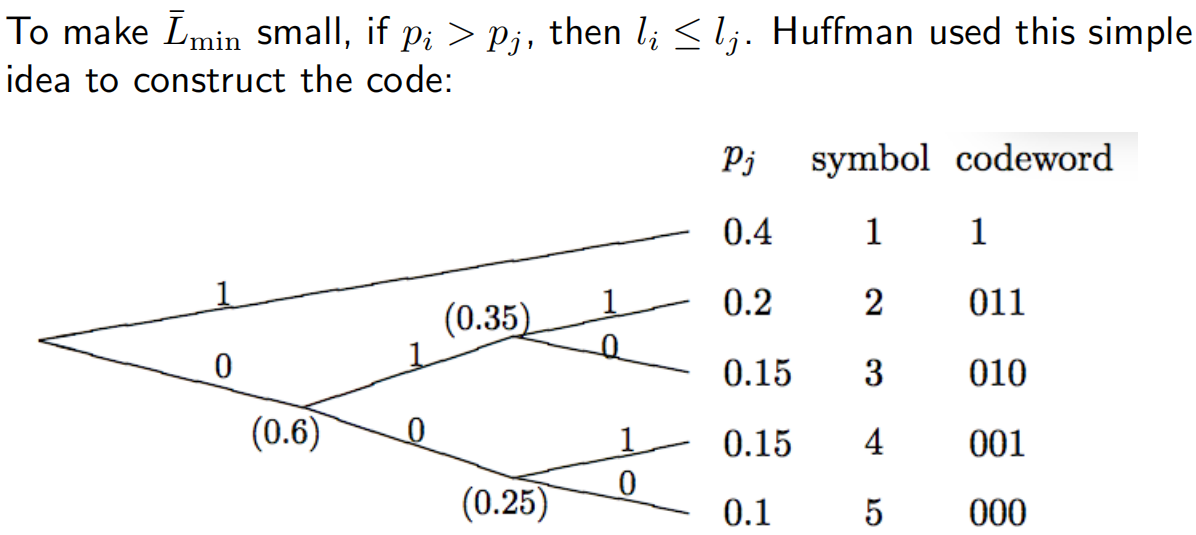
\includegraphics[width=0.8\textwidth]{./figures/chapter3/Huffman.png}
\end{figure}

Huffman 编码可能不唯一. e.g. 两个元素有相同的概率 / 合并时给哪个分支 0, 1 均可.

Property: .

Efficiency of the code: $\eta = \dfrac{H(X)}{L}\leq 1$.

\begin{proposition}
Huffman 编码是最优的(最小的平均码长), 并且满足: \\
1. If $p_i>p_j$, then $l_i\textcolor{red}{\leq} l_j$. \\
2. Optimal prefix-free code has a full tree. \\
3. The two least probable symbols have the same length: 拥有最长编码长度的元素一定至少有2个(否则可以一块剪短一层).
\end{proposition}

Huffman Code for encoding a block: \\
Let $Y=\left(x_1,\ldots,x_n\right)$: $n$ symbol block. \\
假设对 $Y$ 使用Huffman编码, 则平均码长 $\overline{L}_n$ 满足:
$$H(Y)\leq \overline{L}_n < H(Y)+1$$
因为$X_1,\ldots,X_n\stackrel{i.i.d.}{\sim}P_X$, 所以
$$H(Y)=H(X^n)=H(X_1,\ldots,X_n)=\sum_{i=1}^nH(X_i)=nH(X)$$
i.e. 每个 symbol 的平均码长 $\overline{L}=\dfrac{\overline{L}_n}{n}$ 满足:
\begin{align*}
nH(X) &\leq \overline{L}_n < nH(X)+1 \\
\Rightarrow H(X) &\leq \overline{L} < H(X)+\dfrac{1}{n}
\end{align*}


证明 Huffman coding is optimal: 用数学归纳法, 假设有 $M$ 个元素的Huffman编码是最优的 $\to$ 有 $M+1$ 个元素的Huffman编码是最优的.
\begin{figure}[htbp]
    \centering
    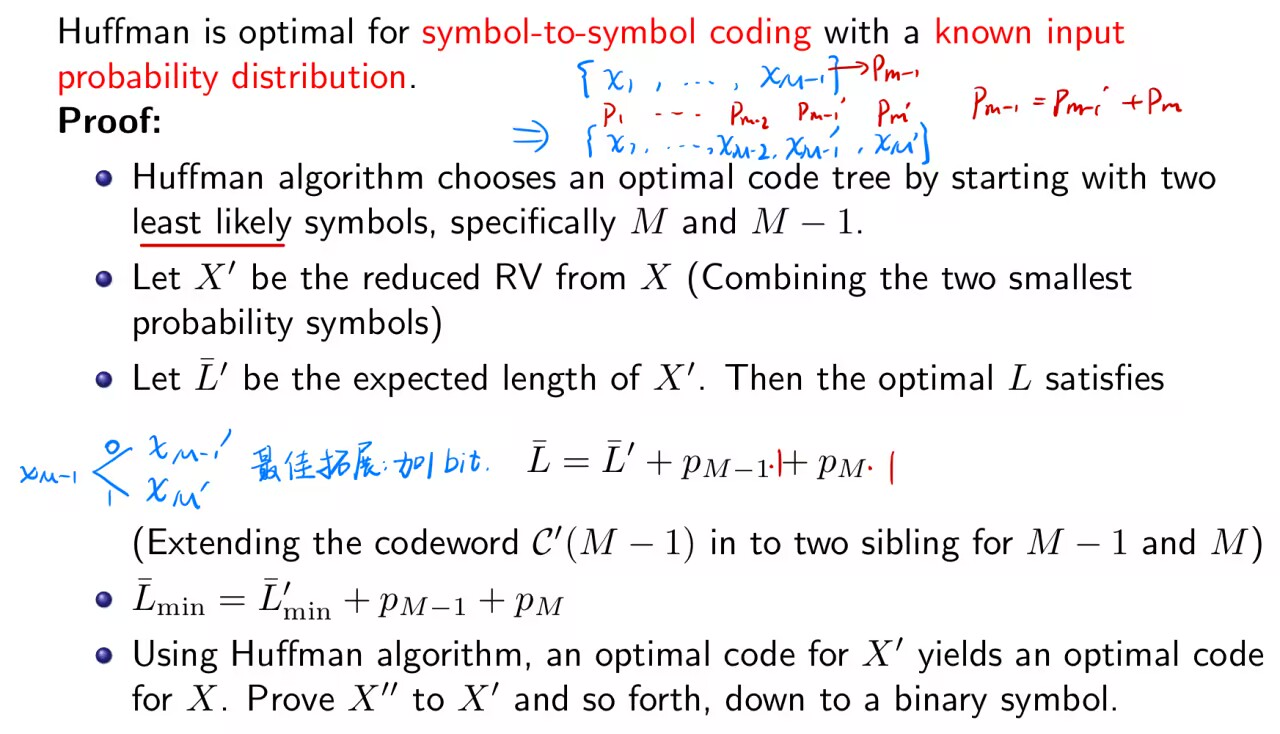
\includegraphics[width=1.1\textwidth]{./figures/chapter3/Huffman_optimal.png}
\end{figure}